\documentclass{article}
\usepackage[italian]{babel}
\usepackage{graphicx}

% permette agli hypertext di essere cliccabili
\usepackage{hyperref}
\usepackage{longtable}

\renewcommand{\arraystretch}{1.6}

\usepackage[raggedrightboxes]{ragged2e}

\usepackage[inline]{enumitem}
\setlist[itemize]{itemsep=0pt, topsep=2pt} % imposta di defualt le opzioni di itemize

\hypersetup{
    colorlinks,
    citecolor=black,
    filecolor=black,
    linkcolor=black,
    urlcolor=black
}
% permette di impostare le dimensioni della pagina
\usepackage[a4paper, total={6in, 9in}]{geometry}

\newcommand{\sskip}{\smallskip \\}
\newcommand{\meskip}{\medskip \\}
\newcommand{\bskip }{\bigskip \\}

\title{Documentazione database\\
Sistema di gestione di personale e progetti all'interno di un'azienda }
\author{Roberto Ingenito \and Simone Ingenito \and Lorenzo Sequino}
\date{\today \\ \vspace{2cm} 
\includegraphics[width=0.5\textwidth]{images/logo.png}}

\begin{document}

\maketitle

\newpage

\tableofcontents

\newpage

\section{Progettazione concettuale}
\subsection{Analisi dei requisiti}
% \raggedright
La base dati si deve occupare della gestione del personale di un'azienda:

la figura centrale di tutto lo schema è l'impiegato.\sskip
La prima classificazione di un generico impiegato viene fatta tra:
\begin{itemize}
	\item impiegato assunto regolarmente
	\item impiegato assunto esclusivamente per lavorare ad un progetto
\end{itemize}\medskip
Gli impiegati assunti regolarmente, vengono assunti con un determinato ruolo e stipendio, inoltre hanno diverse specializzazioni in base sia al merito sia agli anni trascorsi all'interno dell'azienda.

Dal momento in cui viene assunto, l'impiegato diventa automaticamente un junior. Trascorsi 3 anni diventa middle, trascorsi altri 4 diventa senior.
Inoltre, qualunque siano gli anni trascorsi all'interno dell'azienda, può essere promosso e diventare manager.\sskip
Si tiene traccia di tutti gli scatti di carriera all'interno dell'entità \textit{\careerlog} dove sono memorizzati:
\begin{itemize}
	\item ruolo precedente
	\item ruolo successivo
	\item data dello scatto
\end{itemize}\medskip
L'azienda è divisa in varie sedi dove sono presenti diversi laboratori.\sskip
% CONTROLLARE: Un impiegato può lavorare in più laboratori anche contemporaneamente
Ogni impiegato afferisce ad un unico laboratorio.\\
Un impiegato può aver anche lavorato in più laboratori ma in periodi diversi.\\
% -----------
Al momento dell'assunzione l'impiegato non ha ancora una collocazione ma viene stabilita successivamente.\\
Ad un impiegato senior può essere assegnata la gestione di laboratori e/o di progetti.\sskip
Ad ogni laboratorio è assegnato un manager scientifico che è un impiegato senior.\sskip
L'amministratore, a cui è affidata la gestione del database, si occupa di:
\begin{itemize}
	\item inserire gli impiegati assunti
	\item monitorare gli scatti di carriera
	\item promuovere gli impiegati meritevoli a manager
	\item creare progetti e affidare la supervisione ad un manager e la gestione ad un referente scientifico
\end{itemize}\smallskip
Per ogni progetto viene stabilita una data di inizio, una \textit{deadline} per la conclusione del progetto e dei fondi.

Inoltre, si tiene traccia dell'effettiva data in cui il progetto è terminato \textit{end\_date}; può accadere che il progetto si protragga oltre la deadline.\sskip
Ad un progetto possono prendere parte massimo 3 laboratori contemporaneamente.\\
Ogni impiegato che afferisce ad un laboratorio prende parte automaticamente a tutti i progetti a cui quel laboratorio sta lavorando.

Il manager scientifico di un laboratorio decide a quali progetti partecipare e abbandonare, e richiede attrezzatura.\sskip
Le richieste vengono memorizzate nell'entità \textit{\equipmentrequest}.
Queste vengono valutate dal manager e dal referente scientifico del progetto a cui sono state fatte, i quali decidono, in base ai fondi del progetto, se soddisfare le richieste, con il vincolo che il costo totale delle attrezzature non può superare il 50\% dei fondi del progetto.\sskip
Quando viene acquistata dell'attrezzatura, si salva l'acquisto nell'entità \textit{purchase} che tiene traccia della data e del prezzo d'acquisto.\sskip
Ogni attrezzatura di ogni laboratorio viene memorizzata nell'entità \textit{equipment}.\\
Un laboratorio può possedere già dell'attrezzatura (acquistata precedentemente da altri progetti) e riceverne altra tramite richieste a progetti. Di conseguenza l'attrezzatura acquistata in un laboratorio, rimane anche dopo la fine del progetto.\sskip
Con il restante 50\% dei fondi, il manager e il referente scientifico di un progetto possono assumere del personale che viene pagato per lavorare esclusivamente per quel progetto, e non viene considerato come impiegato regolare.

Lo stesso impiegato può essere assunto più volte (anche per lo stesso progetto ma in date differenti), per questo motivo ognuno di questi impiegati non viene rimosso una volta terminato il contratto.
La relazione \textit{\workson} infatti, tiene traccia di tutte le volte in cui un impiegato è stato assunto per lavorare ai progetti.


\subsection{Schema concettuale}\bigskip
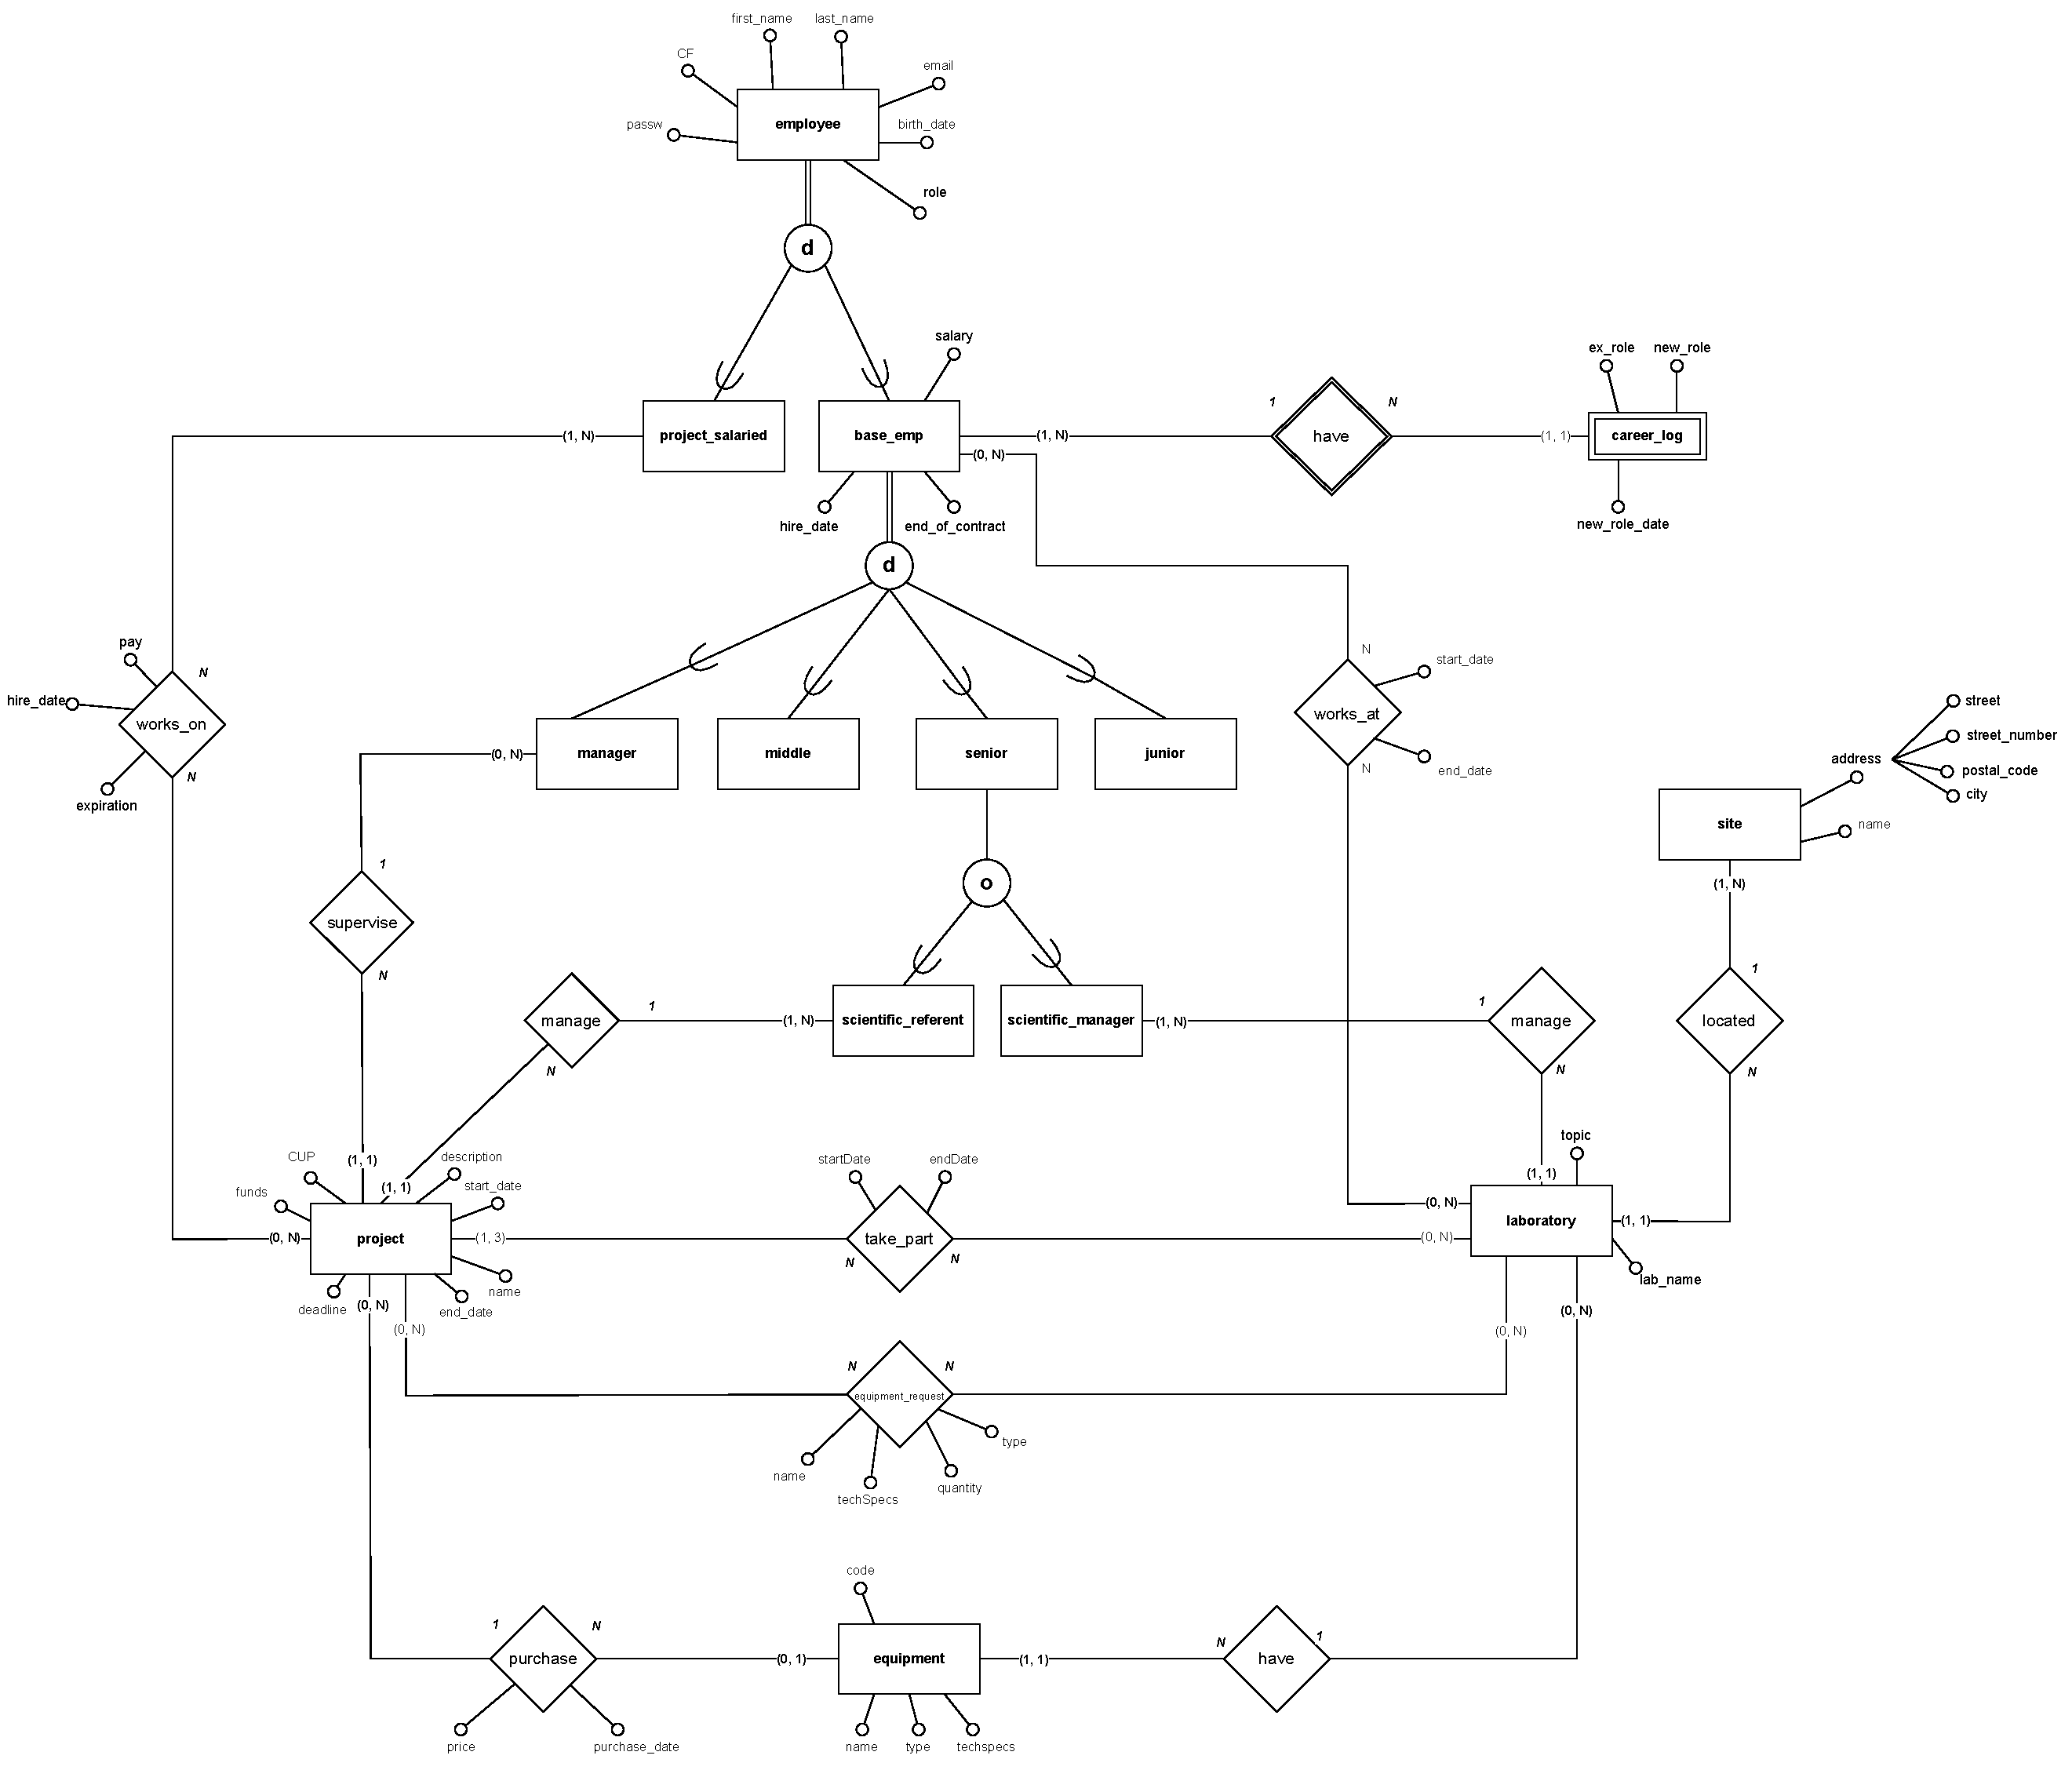
\includegraphics[width=\textwidth]{images/concettualeER.drawio.pdf}

\newpage
\subsection{Dizionario delle entità}
\begin{longtable}{@{}| p{0.2\textwidth} | p{0.4\textwidth} | p{0.3\textwidth} |}
	\hline
	Entità               & Descrizione                                                                                           & Attributi \\
	\hline
	employee             & \begin{minipage}[t]{0.4\textwidth}
		                       \raggedright
		                       Generico impiegato dell'azienda
	                       \end{minipage}
	                     & \begin{minipage}[t]{0.3\textwidth}
		                       \raggedright
		                       \textbf{cf}: Codice fiscale, informazione utile all'azienda\sskip
		                       \textbf{first\_name} \sskip
		                       \textbf{last\_name} \sskip
		                       \textbf{birth\_date} \sskip
		                       \textbf{role}: Professione (sviluppatore, designer, \dots)\sskip
		                       \textbf{email}: Email necessaria per l'accesso al gestionale\sskip
		                       \textbf{passw}: Password necessaria per l'accesso al gestionale
	                       \end{minipage}                                                 \\[140pt]
	\hline
	\baseemp             & \begin{minipage}[t]{0.4\textwidth}
		                       \raggedright
		                       Specializzazione di \textit{employee}. Assunto a tempo indeterminato.
	                       \end{minipage}
	                     & \begin{minipage}[t]{0.3\textwidth}
		                       \raggedright
		                       \textbf{salary}: Stipendio\sskip
		                       \textbf{hire\_date}: Data assunzione
	                       \end{minipage}                                                                               \\[20pt]
	\hline
	\careerlog           & \begin{minipage}[t]{0.4\textwidth}
		                       \raggedright
		                       Entità che memorizza gli scatti di carriera degli impiegati \textit{\baseemp}
	                       \end{minipage}
	                     & \begin{minipage}[t]{0.3\textwidth}
		                       \raggedright
		                       \textbf{ex\_role}: Ruolo precedente (stringa vuota quando è assunto)\sskip
		                       \textbf{new\_role}: Ruolo successivo (stringa vuota quando è licenziato)\sskip
		                       \textbf{new\_role\_date}: Data scatto di carriera
	                       \end{minipage}                                     \\[90pt]
	\hline
	\projectsalaried     & \begin{minipage}[t]{0.4\textwidth}
		                       \raggedright
		                       Specializzazione di \textit{employee}. Assunto per lavorare esclusivamente ad un progetto.
	                       \end{minipage}
	                     &                                                                                                                   \\[25pt]
	\hline
	junior               & \begin{minipage}[t]{0.4\textwidth}
		                       \raggedright
		                       Specializzazione di \textit{\baseemp}. Impiegato che lavora da meno di 3 anni.
	                       \end{minipage}
	                     &                                                                                                                   \\[25pt]
	\hline
	middle               & \begin{minipage}[t]{0.4\textwidth}
		                       \raggedright
		                       Specializzazione di \textit{\baseemp}. Impiegato che lavora dai 4 ai 7 anni.
	                       \end{minipage}
	                     &                                                                                                                   \\[15pt]
	\hline
	senior               & \begin{minipage}[t]{0.4\textwidth}
		                       \raggedright
		                       Specializzazione di \textit{\baseemp}. Impiegato che lavora da più di 7 anni.
	                       \end{minipage}
	                     &                                                                                                                   \\[15pt]
	\hline
	manager              & \begin{minipage}[t]{0.4\textwidth}
		                       \raggedright
		                       Specializzazione di \textit{\baseemp}. Impiegato che ha ricevuto una promozione in base al merito.
	                       \end{minipage}
	                     &                                                                                                                   \\[25pt]
	\hline
	scientific\_referent & \begin{minipage}[t]{0.4\textwidth}
		                       \raggedright
		                       Specializzazione di \textit{senior}. Impiegato a cui è stata affidata la gestione di un progetto.
	                       \end{minipage}
	                     &                                                                                                                   \\[25pt]
	\hline
	scientific\_manager  & \begin{minipage}[t]{0.4\textwidth}
		                       \raggedright
		                       Specializzazione di \textit{senior}.  Impiegato a cui è stata affidata la gestione di un laboratorio.
	                       \end{minipage}
	                     &                                                                                                                   \\[25pt]
	\hline
	project              & \begin{minipage}[t]{0.4\textwidth}
		                       \raggedright
		                       Progetto a cui prendono parte i laboratori e i relativi impiegati.
	                       \end{minipage}
	                     & \begin{minipage}[t]{0.3\textwidth}
		                       \raggedright
		                       \textbf{CUP}: Codice Univoco Progett\sskip
		                       \textbf{name}: Nome del progetto\sskip
		                       \textbf{description}: Descrizione del progetto\sskip
		                       \textbf{start\_date}: Data di inizio del progetto\sskip
		                       \textbf{end\_date}: Data di effettiva fine del progetto\sskip
		                       \textbf{deadline}: Data prevista per la fine del progetto\sskip
		                       \textbf{funds}: Somma di denaro disponibile per l'acquisto di attrezzatura e personale
	                       \end{minipage}                             \\[175pt]
	\hline
	laboratory           & \begin{minipage}[t]{0.4\textwidth}
		                       \raggedright
		                       Luogo all'interno dell'azienda nel quale gli impiegati lavorano ai progetti.
	                       \end{minipage}
	                     & \begin{minipage}[t]{0.3\textwidth}
		                       \raggedright
		                       \textbf{topic}: Campo di studi del laboratorio\sskip
		                       \textbf{lab\_name}: Nome del laboratorio
	                       \end{minipage}                                                               \\[40pt]
	\hline
	site                 & \begin{minipage}[t]{0.4\textwidth}
		                       \raggedright
		                       Sede dell'azienda in cui possono essere presente i laboratori.
	                       \end{minipage}
	                     & \begin{minipage}[t]{0.3\textwidth}
		                       \raggedright
		                       \textbf{name}: Nome della sede\sskip
		                       \textbf{address}: Indirizzo
		                       \begin{itemize}
			\item \textbf{street}: Via
			\item \textbf{street\_number}: Numero civico
			\item \textbf{postal\_code}: CAP
			\item \textbf{city}: Città
		\end{itemize}
	                       \end{minipage}                                                                               \\[90pt]
	\hline
	equipment            & \begin{minipage}[t]{0.4\textwidth}
		                       \raggedright
		                       Attrezzatura presente all'interno di un laboratorio
	                       \end{minipage}
	                     & \begin{minipage}[t]{0.3\textwidth}
		                       \raggedright
		                       \textbf{code}: Codice del prodotto\sskip
		                       \textbf{name}: Nome del prodotto\sskip
		                       \textbf{type}: Tipo di prodotto (computer, microscopio, \dots)\sskip
		                       \textbf{techspecs}: Specifiche tecniche del prodotto
	                       \end{minipage}                                               \\[70pt]
	\hline
\end{longtable}

\newpage
\subsection{Dizionario delle associazioni}
\begin{tabular}{@{}| p{0.2\textwidth} | p{0.4\textwidth} | p{0.3\textwidth} |}
	\hline
	Associazioni      & Descrizione                                                                               & Attributi \\
	\hline
	\workson          & \begin{minipage}[t]{0.4\textwidth}
		                    \raggedright
		                    Associazione tra \textit{\projectsalaried} e \textit{project} \textbf{molti-a-molti}
	                    \end{minipage}      & \begin{minipage}[t]{0.3\textwidth}
		                                          \raggedright
		                                          \textbf{pay}: Paga stabilita per lavorare a quel progetto\sskip
		                                          \textbf{hire\_date}: Data di assunzione\sskip
		                                          \textbf{expiration}: Data di fine contratto
	                                          \end{minipage}
	\\[70pt]
	\hline
	\worksat          & \begin{minipage}[t]{0.4\textwidth}
		                    \raggedright
		                    Associazione tra \textit{\baseemp} e \textit{laboratory} \textbf{molti-a-molti}.
	                    \end{minipage}
	                  & \begin{minipage}[t]{0.3\textwidth}
		                    \raggedright
		                    \textbf{start\_date}: Data di assegnazione di un impiegato ad un laboratorio\sskip
		                    \textbf{end\_date}: Data di fine lavoro
	                    \end{minipage}                     \\[55pt]
	\hline
	supervise         & \begin{minipage}[t]{0.4\textwidth}
		                    \raggedright
		                    Associazione tra \textit{manager} e \textit{project} \textbf{uno-a-molti}.
	                    \end{minipage}
	                  &                                                                                                       \\[15pt]
	\hline
	manage            & \begin{minipage}[t]{0.4\textwidth}
		                    \raggedright
		                    Associazione tra \textit{scientific\_referent} e \textit{project} \textbf{uno-a-molti}.
	                    \end{minipage}
	                  &                                                                                                       \\[15pt]
	\hline
	manage            & \begin{minipage}[t]{0.4\textwidth}
		                    \raggedright
		                    Associazione tra \textit{scientific\_manager} e \textit{laboratory} \textbf{uno-a-molti}.
	                    \end{minipage}
	                  &                                                                                                       \\[15pt]
	\hline
	\takepart         & \begin{minipage}[t]{0.4\textwidth}
		                    \raggedright
		                    Associazione tra \textit{project} e \textit{laboratory} \textbf{molti-a-molti}.
	                    \end{minipage}
	                  & \begin{minipage}[t]{0.3\textwidth}
		                    \raggedright
		                    \textbf{start\_date}: Data in cui un laboratorio inizia a lavorare ad un progetto \sskip
		                    \textbf{end\_date}: Data di fine lavoro
	                    \end{minipage}               \\[55pt]
	\hline
	purchase          & \begin{minipage}[t]{0.4\textwidth}
		                    \raggedright
		                    Associazione tra \textit{project} e \textit{equipment} \textbf{uno-a-molti}.
	                    \end{minipage}              & \begin{minipage}[t]{0.3\textwidth}
		                                                  \raggedright
		                                                  \textbf{purchase\_date}: Data di acquisto\sskip
		                                                  \textbf{price}: Prezzo dell'attrezzatura
	                                                  \end{minipage}                          \\[40pt]
	\hline
	\equipmentrequest & \begin{minipage}[t]{0.4\textwidth}
		                    \raggedright
		                    Associazione tra \textit{project} e \textit{laboratory} \textbf{molti-a-molti}.
	                    \end{minipage}
	                  &                                                                                                       \\[15pt]
	\hline
	have              & \begin{minipage}[t]{0.4\textwidth}
		                    \raggedright
		                    Associazione tra \textit{equipment} e \textit{laboratory} \textbf{uno-a-molti}.
	                    \end{minipage}
	                  &                                                                                                       \\[15pt]
	\hline
	have              & \begin{minipage}[t]{0.4\textwidth}
		                    \raggedright
		                    Associazione tra \textit{\baseemp} e \textit{\careerlog} \textbf{uno-a-molti}.
	                    \end{minipage}
	                  &                                                                                                       \\[15pt]
	\hline
	located           & \begin{minipage}[t]{0.4\textwidth}
		                    \raggedright
		                    Associazione tra \textit{site} e \textit{laboratory} \textbf{uno-a-molti}.
	                    \end{minipage}
	                  &                                                                                                       \\[15pt]
	\hline
\end{tabular}


\section{Ristrutturazione del modello concettuale}
\subsection{Analisi delle ridondanze}
È presente una ridondanza nel campo \textit{hire\_date} di \textit{base\_emp} in quanto è possibile calcolarla dall'entità associata \textit{career\_log}
\subsection{Eliminazione degli attributi multivalore}
Non sono presenti attributi multivalore
\subsection{Eliminazione degli attributi composti}
L'attributo \textit{address} di \textit{site} è un attributo composto.

Siccome l'indirizzo è unico per ogni sede, si è deciso di accorpare gli attributi di \textit{address} in \textit{site}.\meskip
L'attributo \textit{tech\_specs} di \textit{equipment} potrebbe essere scomposto in più attributi ma in questo caso non è necessario ai fini della traccia, quindi è più comodo memorizzarlo come un unico campo stringa.

\subsection{Analisi delle generalizzazioni}
Procediamo all'eliminazione delle generalizzazioni partendo dal basso:
\begin{enumerate}
	\item Accorpamento di \textit{scientific\_referent} e \textit{scientific\_manager} in \textit{senior} in quanto non avendo attributi non è possibile inserire valori nulli che occupano spazio inutile.\\
	      Fatta tale scelta bisogna cambiare la cardinalità da $\;(1, n)\;$ a $\;(0, n)\;$ in entrambe le associazioni, poiché un \textit{senior} può anche non essere nessuno dei due o uno soltanto (overlapping parziale)
	\item Accorpamento di \textit{junior}, \textit{middle}, \textit{senior}, \textit{manager} all'interno di \textit{base\_emp} aggiungendo un attributo che ne specifica il tipo.\\
	      Notare che questa scelta aggiunge una \textbf{ridondanza} poiché il tipo è reperibile effettuando un'interrogazione in \textit{career\_log}. Nonostante ciò è più efficiente e immediato eseguire determinate operazioni avendo quest'attributo disponibile direttamente in \textit{base\_emp}
	\item Accorpamento di \textit{employee} all'interno di \textit{project\_salaried} e \textit{base\_emp} in quanto la generalizzazione è totale.
\end{enumerate}
\subsection{Identificazioni chiavi primarie}
\begin{itemize}
	\item In \textit{base\_emp} abbiamo l'attributo \textit{CF} (Codice Fiscale), una stringa di $16$ caratteri
	\item In \textit{project\_salaried} abbiamo l'attributo \textit{CF} (Codice Fiscale), una stringa di $16$ caratteri
	\item \textit{project} è identificato dal \textit{CUP} (Codice Univoco Progetto)
	\item \textit{equipment} è identificato da \textit{code} che è un codice generato randomicamente
	\item \textit{equipment\_request} è identificato da \textit{code} che è un codice generato randomicamente
	\item \textit{site} è identificato da un nuovo attributo \textit{site\_number} che si autoincrementa
	\item \textit{laboratory} è identificato da un nuovo attributo \textit{lab\_code} che si autoincrementa
\end{itemize}
\newpage

\subsection{Schema ristrutturato UML}
\bigskip 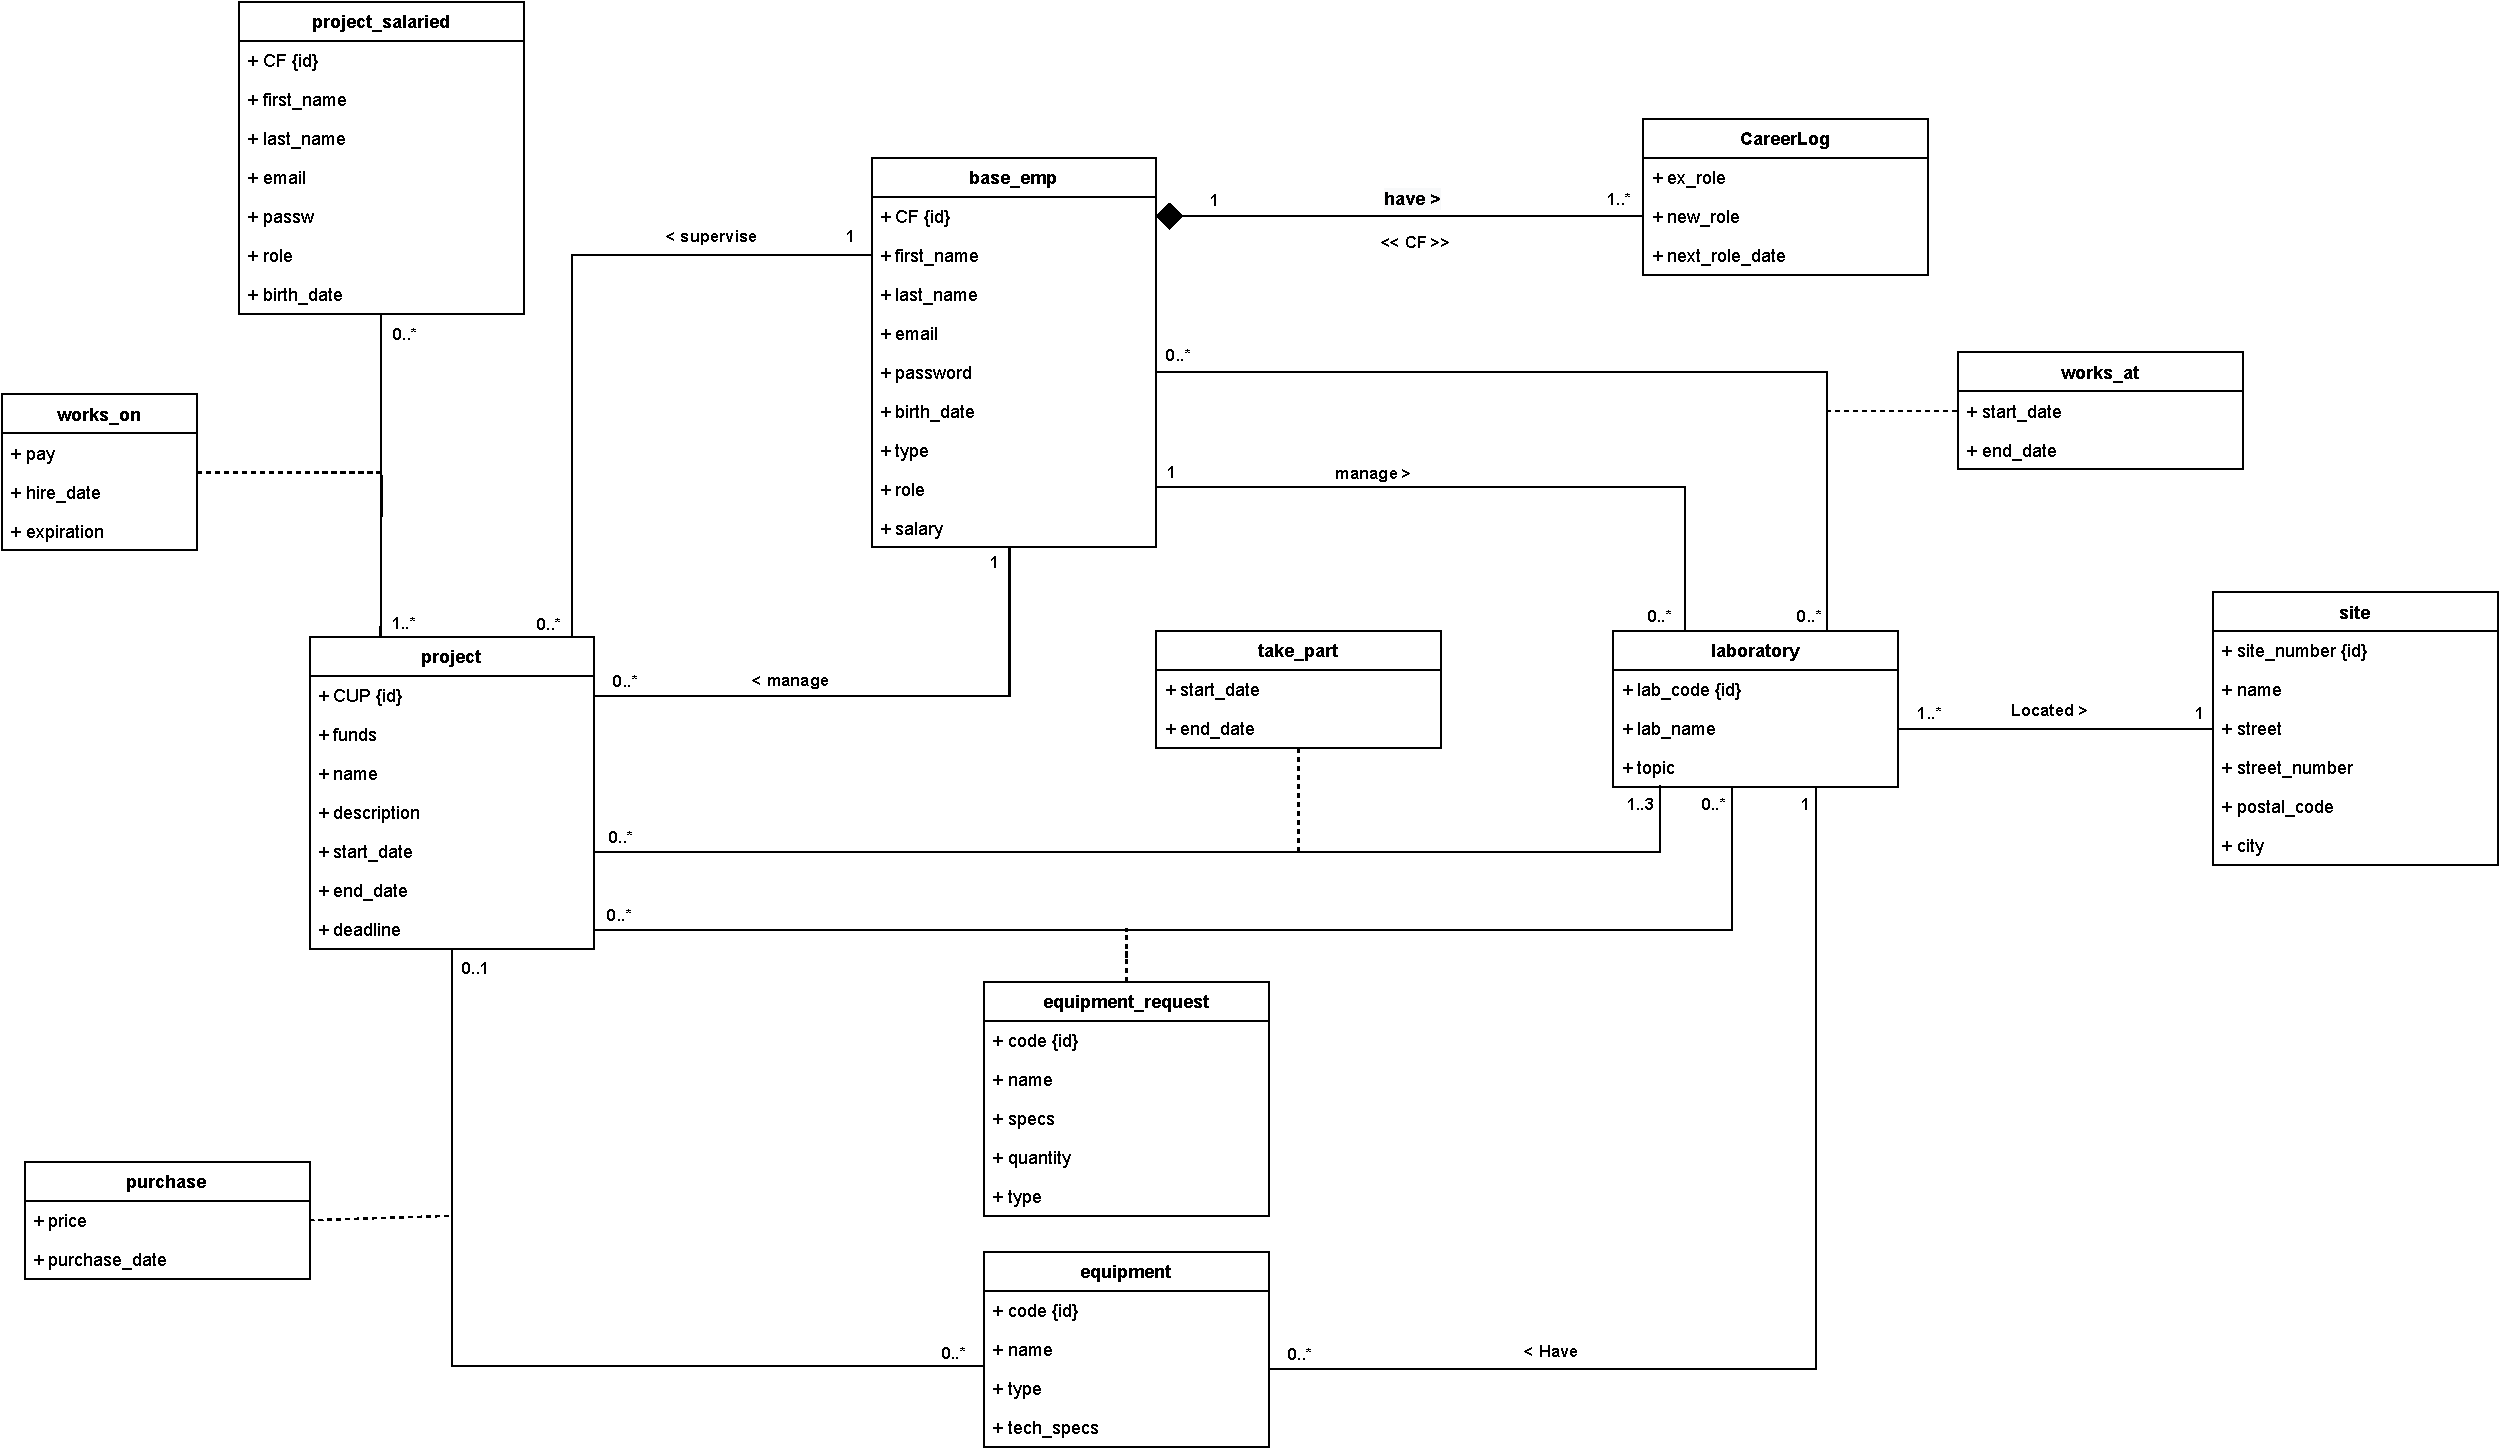
\includegraphics[width=\textwidth]{images/Ristrutturato-UML.drawio.pdf}


\subsection{Schema ristrutturato ER}
\bigskip 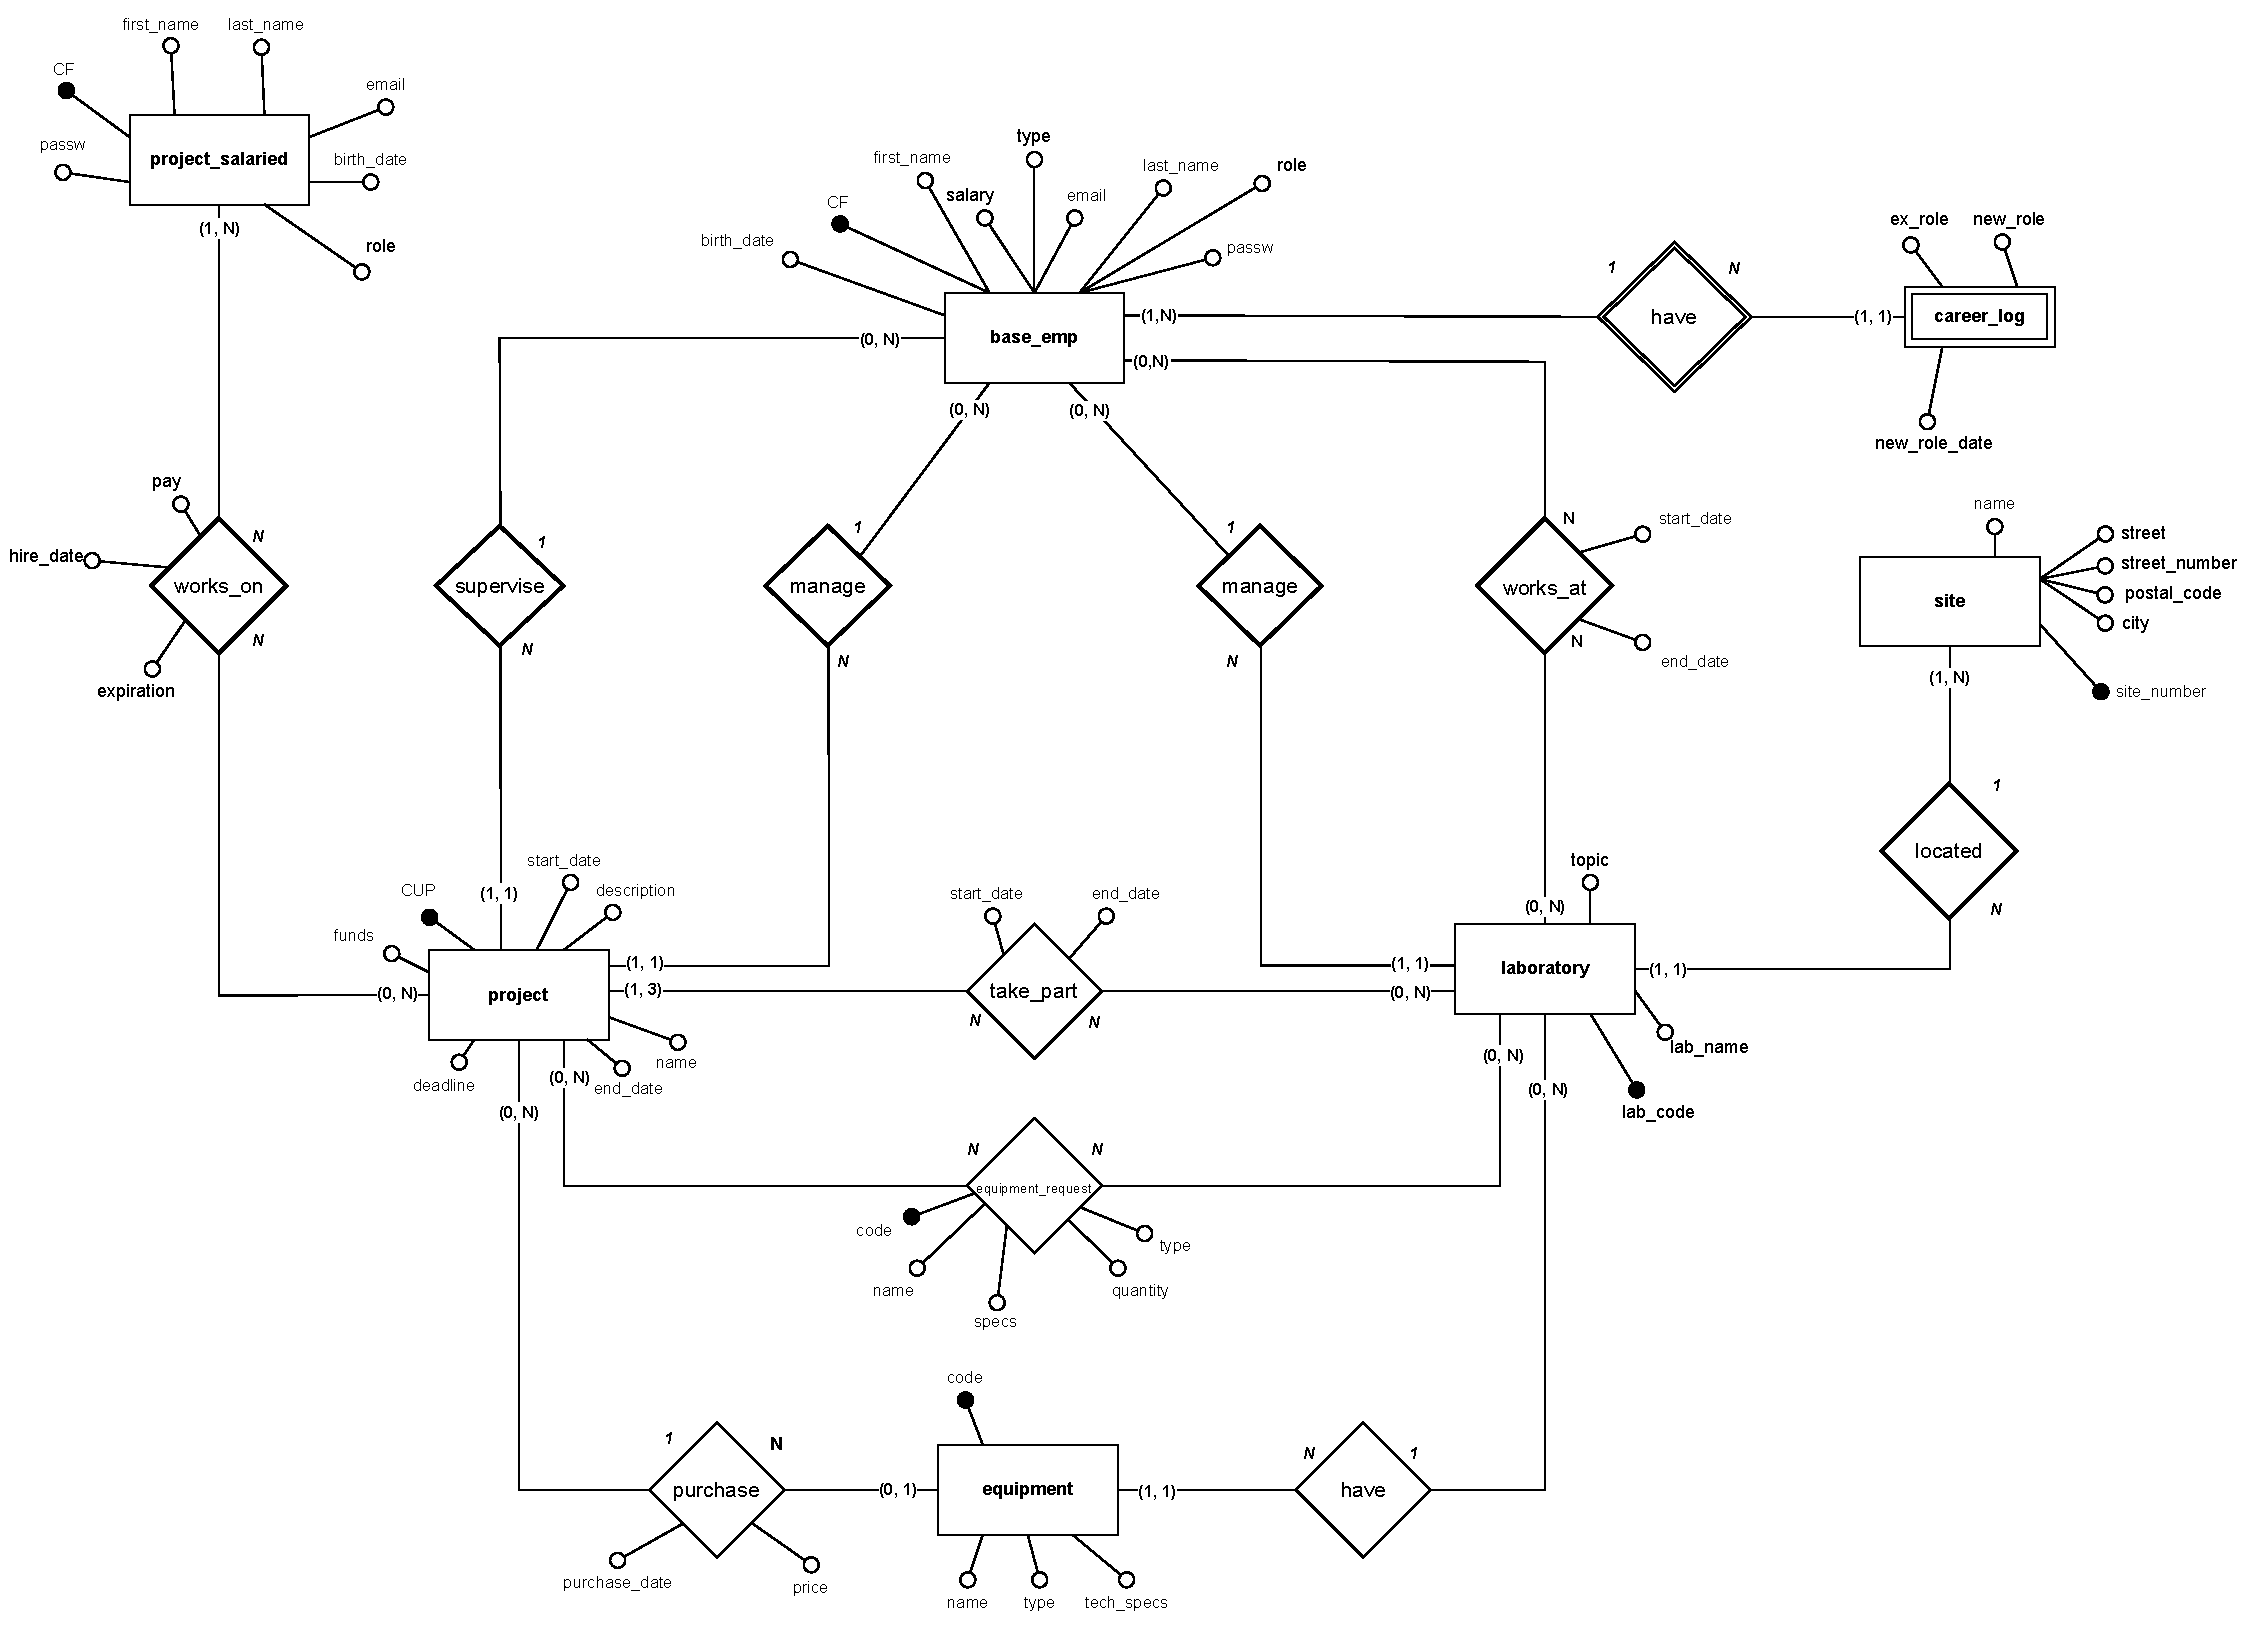
\includegraphics[width=\textwidth]{images/Ristrutturato-ER.drawio.pdf}




\section{Traduzione al modello logico}
\subsection{Mapping associazioni}
\subsubsection{Associazioni 1-N}
\begin{itemize}
	\item \textit{Site} - \textit{Located} - \textit{Laboratory}:  inserimento chiave di \textit{Site} in \textit{Laboratory} come chiave esterna
	\item \textit{base\_emp} - \textit{Supervise} - \textit{Project}: inserimento chiave di \textit{base\_emp} all'interno di \textit{Project} come chiave esterna
	\item \textit{base\_emp} - \textit{Manage} - \textit{Project}: inserimento chiave di \textit{base\_emp} all'interno di \textit{Project} come chiave esterna
	\item \textit{base\_emp} - \textit{Manage} - \textit{Laboratory}: inserimento di chiave di \textit{base\_emp} all'interno di \textit{Laboratory} come chiave esterna
	\item \textit{Laboratory} - \textit{Have} - \textit{Equipment}: inserimento di chave di \textit{Laboratory} in \textit{Equipment} come chiave esterna
	\item \textit{Project} - \textit{Purchase} - \textit{Equipment}: Equipment ha una partecipazione parziale, si procede come N-N
	\item \textit{base\_emp} - \textit{Have} - \textit{career\_log}: relazione identificante, inserimento di chiave primaria di \textit{base\_emp} in \textit{career\_log} come chiave esterna
\end{itemize}
\subsubsection{Associazioni N-N}
Per ognuna di queste relazioni, si inseriscono le chiavi delle due associazioni come chiavi esterne.\meskip
\begin{tabular}{@{}| l | l | l |}
	\hline
	\textbf{Associazione} & \textbf{Relazione} & \textbf{Associazione} \\
	\hline
	project\_salaried     & works\_on          & project               \\
	\hline
	project               & take\_part         & laboratory            \\
	\hline
	project               & equipment\_request & laboratory            \\
	\hline
	base\_emp             & works\_at          & laboratory            \\
	\hline
\end{tabular}

\newpage
\subsection{Modello logico}
Gli attributi \underline{sottolineati} sono chiavi primarie,\\
gli attributi con un asterisco * alla fine sono chiavi esterne\meskip
\begin{tabular}{@{}l l}
	\textbf{\textit{base\_emp}}          & (\underline{CF}, first\_name, last\_name, email, passw, birth\_date, type, role, salary)                  \\
	\textbf{\textit{career\_log}}        & \makecell[lt]{(\underline{lab\_code}, lab\_name, topic, cf\_scientific\_manager*, site\_number*)          \\
	cf\_scientific\_manager $\mapsto$ base\_emp.CF                                                                                                   \\
	site\_number $\mapsto$ site.site\_number}                                                                                                        \\
	\textbf{\textit{laboratory}}         & \makecell[lt]{(\underline{lab\_code}, lab\_name, topic, cf\_scientific\_manager*, site\_number*)          \\
	cf\_scientific\_manager $\mapsto$ base\_emp.CF                                                                                                   \\
	site\_number $\mapsto$ site.site\_number}                                                                                                        \\
	\textbf{\textit{take\_part}}         & \makecell[lt]{(start\_date, end\_date, CUP*, lab\_code*)                                                  \\
	CUP $\mapsto$ project.CUP                                                                                                                        \\
	lab\_code $\mapsto$ laboratory.lab\_code}                                                                                                        \\
	\textbf{\textit{project}}            & \makecell[lt]{(\underline{CUP}, funds, name, description, start\_date, end\_date, deadline, cf\_manager*, \\
	cf\_scientific\_referent*)                                                                                                                       \\
	cf\_manager $\mapsto$ base\_emp.CF                                                                                                               \\
	cf\_scientific\_referent $\mapsto$ base\_emp.CF}                                                                                                 \\
	\textbf{\textit{project\_salaried}}  & \makecell[lt]{(\underline{CF}, first\_name, last\_name, email, passw, birth\_date, role)}                 \\
	\textbf{\textit{works\_on}}          & \makecell[lt]{(pay, hire\_date, expiration, CF*, CUP*)                                                    \\
	CF $\mapsto$ project\_salaried.CF                                                                                                                \\
	CUP $\mapsto$ project.CUP}                                                                                                                       \\
	\textbf{\textit{site}}               & \makecell[lt]{(\underbar{site\_number}, name, street, street\_number, postal\_code, city)}                \\
	\textbf{\textit{equipment}}          & \makecell[lt]{(\underline{code}, name, type, tech\_specs, lab\_code*)                                     \\
	lab\_code $\mapsto$ laboratory.lab\_code}                                                                                                        \\
	\textbf{\textit{purchase}}           & \makecell[lt]{(purchase\_date, price, CUP*, equipment\_code*)                                             \\
	CUP $\mapsto$ project.CUP                                                                                                                        \\
	equipment\_code $\mapsto$ equipment.code}                                                                                                        \\
	\textbf{\textit{works\_at}}          & \makecell[lt]{(start\_date, end\_date, cf\_base\_emp*, lab\_code*)                                        \\
	cf\_base\_emp $\mapsto$ base\_emp.CF                                                                                                             \\
	lab\_code $\mapsto$ laboratory.lab\_code}                                                                                                        \\
	\textbf{\textit{equipment\_request}} & \makecell[lt]{(\underline{code}, type, name, specs, quantity,  CUP*, lab\_code*)                          \\
	CUP $\mapsto$ project.CUP                                                                                                                        \\
	lab\_code $\mapsto$ laboratory.lab\_code}                                                                                                        \\
\end{tabular}



\section{Progettazione fisica}
\subsection{Creazione del database}
\begin{lstlisting}
CREATE DATABASE company WITH OWNER postgres;
\end{lstlisting}

\subsection{Creazione dello schema}
\begin{lstlisting}
CREATE SCHEMA projects_schema;
\end{lstlisting}

\subsection{Attivazione estensioni}
Le estensioni possono essere attivate solo da un superuser (\textit{postgres} in questo caso); \textit{project\_admin} non può essere superuser altrimenti avrebbe gli stessi privilegi di \textit{postgres}.

Le estensioni vengono create sullo schema \textit{projects\_schema} così che l'utente \textit{project\_admin} ne abbia l'accesso.\meskip
Estensione utilizzata per la cifratura delle password, usata per l'autenticazione lato client.
\lstinputlisting{../basi_di_dati/extension/enable_crypt.sql}\medskip
Estensione utilizzata per generare codici univoci causali.
\lstinputlisting{../basi_di_dati/extension/enable_uuid.sql}

\subsection{Gestione ruoli e permessi}

\subsection{Creazione domini}
\lstinputlisting{../basi_di_dati/domains/cf_type.sql}
\lstinputlisting{../basi_di_dati/domains/cup_type.sql}
\lstinputlisting{../basi_di_dati/domains/emp_type.sql}
\lstinputlisting{../basi_di_dati/domains/equipment_name_type.sql}
\lstinputlisting{../basi_di_dati/domains/name_type.sql}
\lstinputlisting{../basi_di_dati/domains/password_type.sql}
\lstinputlisting{../basi_di_dati/domains/salary_type.sql}

\subsection{Creazione tabelle}
\noindent \textbf{Tabella \baseemp}
\lstinputlisting[lastline=14]{../basi_di_dati/create_tables/base_emp.sql}\bigskip

\noindent \textbf{Tabella \careerlog}
\lstinputlisting[lastline=33]{../basi_di_dati/create_tables/career_log.sql}\bigskip

\noindent \textbf{Tabella laboratory}
\lstinputlisting{../basi_di_dati/create_tables/laboratory.sql}\bigskip

\noindent \textbf{Tabella \takepart}
\lstinputlisting{../basi_di_dati/create_tables/take_part.sql}\bigskip

\noindent \textbf{Tabella \projectsalaried}
\lstinputlisting{../basi_di_dati/create_tables/project_salaried.sql}\bigskip

\noindent \textbf{Tabella \workson}
\lstinputlisting{../basi_di_dati/create_tables/works_on.sql}\bigskip

\noindent \textbf{Tabella site}
\lstinputlisting{../basi_di_dati/create_tables/site.sql}\bigskip

\noindent \textbf{Tabella equipment}
\lstinputlisting{../basi_di_dati/create_tables/equipment.sql}\bigskip

\noindent \textbf{Tabella purchase}
\lstinputlisting{../basi_di_dati/create_tables/purchase.sql}\bigskip

\noindent \textbf{Tabella \worksat}
\lstinputlisting{../basi_di_dati/create_tables/works_at.sql}\bigskip

\noindent \textbf{Tabella \equipmentrequest}
\lstinputlisting{../basi_di_dati/create_tables/equipment_request.sql}\bigskip

\noindent \textbf{Tabella project}
\lstinputlisting{../basi_di_dati/create_tables/project.sql}\bigskip

\subsection{Trigger e trigger function}

\subsection{Procedure e funzioni}

\subsection{Dizionario dei vincoli}
\subsubsection{Vincoli intra-relazionali}
\begin{tabular}{@{}| p{.3\textwidth} | p{.6\textwidth} |@{}} % base emp
	\hline
	\multicolumn{2}{|c|}{\textbf{\baseemp}}         \\
	\hline
	\textbf{Vincolo}   & \textbf{Descrizione}       \\
	\hline
	emp\_email\_unique & L'email è univoca          \\
	\hline

	\baseemp\_pk       & Vincolo di chiave primaria \\
	\hline
\end{tabular}\bskip
\begin{tabular}{@{}| p{.3\textwidth} | p{.6\textwidth} |@{}} % laboratory
	\hline
	\multicolumn{2}{|c|}{\textbf{laboratory}}                \\
	\hline
	\textbf{Vincolo}            & \textbf{Descrizione}       \\
	\hline
	lab\_pk                     & Vincolo di chiave primaria \\
	\hline
	site\_number\_fk            & Vincolo di chiave esterna  \\
	\hline
	cf\_scientific\_manager\_fk & Vincolo di chiave esterna  \\
	\hline
\end{tabular}\bskip
\begin{tabular}{@{}| p{.3\textwidth} | p{.6\textwidth} |@{}} % career log 
	\hline
	\multicolumn{2}{|c|}{\textbf {\careerlog}}                                                                                                     \\
	\hline
	\textbf{Vincolo}  & \textbf{Descrizione}                                                                                                       \\
	\hline
	emp\_career\_fk   & \begin{minipage}[t]{.6\textwidth}
		                    Vincolo di chiave esterna.\\
		                    Se viene eliminato l'impiegato, verrà eliminata anche la tupla in \textit{\careerlog}

	                    \end{minipage}                                       \\[26pt]
	\hline
	check\_new\_grade & \begin{minipage}[t]{.6\textwidth}
		                    Controlla che gli scatti di carriera siano coerenti.\\
		                    Ad esempio non è possibile passare da \textit{junior} a \textit{senior} senza essere diventati prima \textit{middle}.\sskip
		                    La stringa vuota come primo parametro significa che l'impiegato è stato assunto;\\
		                    come secondo invece, significa che è stato licenziato.\meskip
		                    \textbf{Casi possibili:}
		                    \begin{itemize}
			\item (' ', 'junior')
			\item ('junior', 'middle')
			\item ('middle', 'senior') \medskip
			\item ('junior', 'manager')
			\item ('middle', 'manager')
			\item ('senior', 'manager') \medskip
			\item ('manager', 'junior')
			\item ('manager', 'middle')
			\item ('manager', 'senior') \medskip
			\item ('junior', ' ')
			\item ('middle', ' ')
			\item ('senior', ' ')
			\item ('manager', ' ')

		\end{itemize}

	                    \end{minipage} \\[310pt]
	\hline
\end{tabular}\bskip
\begin{tabular}{@{}| p{.3\textwidth} | p{.6\textwidth} |@{}} % equipment request
	\hline
	\multicolumn{2}{|c|}{\textbf{\equipmentrequest}}                                                                                                             \\
	\hline
	\textbf{Vincolo}       & \textbf{Descrizione}                                                                                                                \\
	\hline
	equipment\_request\_pk & Vincolo di chiave primaria                                                                                                          \\
	\hline
	CUP\_fk                & \begin{minipage}[t]{.6\textwidth}
		                         \raggedright
		                         Vincolo di chiave esterna.\\
		                         Se viene eliminato il progetto (o modificato il cup), verrà eliminata (o aggiornata) anche la tupla in \textit{\equipmentrequest}
	                         \end{minipage}    \\[40pt]
	\hline
	lab\_code\_fk          & \begin{minipage}[t]{.6\textwidth}
		                         \raggedright
		                         Vincolo di chiave esterna.\\
		                         Se viene eliminato il laboratorio (o modificato il cup), verrà eliminata (o aggiornata) anche la tupla in \textit{\equipmentrequest}
	                         \end{minipage} \\[40pt]
	\hline
	check\_quantity        & Controlla che la quantità sia maggiore di $0$                                                                                       \\
	\hline
\end{tabular}\bskip
\begin{tabular}{@{}| p{.3\textwidth} | p{.6\textwidth} |@{}} % equipment
	\hline
	\multicolumn{2}{|c|}{\textbf{equipment}}                                                                          \\
	\hline
	\textbf{Vincolo} & \textbf{Descrizione}                                                                           \\
	\hline
	equipment\_pk    & Vincolo di chiave primaria                                                                     \\
	\hline
	lab\_code\_fk    & \begin{minipage}[t]{.6\textwidth}
		                   \raggedright
		                   Vincolo di chiave esterna.\\
		                   Se viene eliminato il laboratorio, la chiave esterna verrà posta a NULL.\\
		                   Se viene aggiornata la chiave di \textit{laboratory}, verrà aggiornata anche la chiave esterna.
	                   \end{minipage} \\[50pt]
	\hline
\end{tabular}\bskip
\begin{tabular}{@{}| p{.3\textwidth} | p{.6\textwidth} |@{}} % project salaried
	\hline
	\multicolumn{2}{|c|}{\textbf{\projectsalaried}}   \\
	\hline
	\textbf{Vincolo}     & \textbf{Descrizione}       \\
	\hline
	\projectsalaried\_pk & Vincolo di chiave primaria \\
	\hline
	emp\_email\_unique   & L'email è univoca          \\
	\hline
\end{tabular}\bskip
\begin{tabular}{@{}| p{.3\textwidth} | p{.6\textwidth} |@{}} % project
	\hline
	\multicolumn{2}{|c|}{\textbf{project}}                                                                         \\
	\hline
	\textbf{Vincolo}             & \textbf{Descrizione}                                                            \\
	\hline
	project\_pk                  & Vincolo di chiave primaria                                                      \\
	\hline
	check\_deadline              & Verifica che la deadline sia dopo la data di inizio (nel caso in cui ci fosse). \\
	\hline
	check\_end\_date             & Verifica che la data di fine progetto sia dopo la data di inizio.               \\
	\hline
	fk\_cf\_manager              & Vincolo di chiave esterna                                                       \\
	\hline
	fk\_cf\_scientific\_referent & Vincolo di chiave esterna                                                       \\
	\hline
\end{tabular}\bskip
\begin{tabular}{@{}| p{.3\textwidth} | p{.6\textwidth} |@{}} % purchase
	\hline
	\multicolumn{2}{|c|}{\textbf{purchase}}                                                                                                                                 \\
	\hline
	\textbf{Vincolo}    & \textbf{Descrizione}                                                                                                                              \\
	\hline
	cup\_type\_fk       & Vincolo di chiave esterna.

	Se viene eliminato il progetto, la chiave esterna viene posta a NULL, questo perché si vuole tenere traccia della data d'acquisto e del prezzo dell'attrezzatura.       \\
	\hline
	equipment\_code\_fk & Vincolo di chiave esterna.

	Se viene eliminato l'attrezzatura, verrà eliminata anche la tupla in purchase, dato che diventa inutile tenere traccia dell'acquisto di un prodotto che non si conosce. \\
	\hline
	check\_price        & Controlla che il prezzo sia maggiore di $0$                                                                                                       \\
	\hline
\end{tabular}\bskip
\begin{tabular}{@{}| p{.3\textwidth} | p{.6\textwidth} |@{}} % site
	\hline
	\multicolumn{2}{|c|}{\textbf{site}}           \\
	\hline
	\textbf{Vincolo} & \textbf{Descrizione}       \\
	\hline
	site\_pk         & Vincolo di chiave primaria \\
	\hline
\end{tabular}\bskip
\begin{tabular}{@{}| p{.3\textwidth} | p{.6\textwidth} |@{}} % take part
	\hline
	\multicolumn{2}{|c|}{\textbf{\takepart}}                                                                                                             \\
	\hline
	\textbf{Vincolo} & \textbf{Descrizione}                                                                                                              \\
	\hline
	date\_integrity  & Verifica che la data in cui il laboratorio termina di lavorare al progetto, sia dopo la data di inizio.                           \\
	\hline
	CUP\_fk          & \begin{minipage}[t]{.6\textwidth}
		                   \raggedright
		                   Vincolo di chiave esterna.\\
		                   Se viene eliminato il progetto (o modificato il cup), verrà eliminata (o aggiornata) anche la tupla in \textit{\takepart}
	                   \end{minipage}          \\[27pt]
	\hline
	lab\_code\_fk    & \begin{minipage}[t]{.6\textwidth}
		                   \raggedright
		                   Vincolo di chiave esterna.\\
		                   Se viene eliminato il laboratorio (o modificato il lab\_code), verrà eliminata (o aggiornata) anche la tupla in \textit{\takepart}
	                   \end{minipage} \\[36pt]
	\hline
\end{tabular}\bskip
\begin{tabular}{@{}| p{.3\textwidth} | p{.6\textwidth} |@{}} % works at
	\hline
	\multicolumn{2}{|c|}{\textbf{\worksat}}                                                                                                              \\
	\hline
	\textbf{Vincolo}  & \textbf{Descrizione}                                                                                                             \\
	\hline
	date\_integrity   & Verifica che la data in cui l'impiegato termina di lavorare al laboratorio, sia dopo la data di inizio.                          \\
	\hline
	cf\_base\_emp\_fk & \begin{minipage}[t]{.6\textwidth}
		                    \raggedright
		                    Vincolo di chiave esterna.\\
		                    Se viene eliminato l'impiegato (o modificato il cf), verrà eliminata (o aggiornata) anche la tupla in \textit{\worksat}
	                    \end{minipage}           \\[27pt]
	\hline
	lab\_code\_fk     & \begin{minipage}[t]{.6\textwidth}
		                    \raggedright
		                    Vincolo di chiave esterna.\\
		                    Se viene eliminato il laboratorio (o modificato il lab\_code), verrà eliminata (o aggiornata) anche la tupla in \textit{\worksat}
	                    \end{minipage} \\[36pt]
	\hline
\end{tabular}\bskip
\begin{tabular}{@{}| p{.3\textwidth} | p{.6\textwidth} |@{}} % works on
	\hline
	\multicolumn{2}{|c|}{\textbf{\workson}}                                                          \\
	\hline
	\textbf{Vincolo}        & \textbf{Descrizione}                                                   \\
	\hline
	check\_expiration\_date & Verifica che la data di fine contratto sia dopo la data di assunzione. \\
	\hline
	fk\_cf                  & Vincolo di chiave esterna.

	Se viene eliminato l'impiegato, verrà posta la chiave esterna a NULL.

	Questo perché si vuole salvare i contratti anche se un impiegato a progetto viene eliminato.     \\
	\hline
	fk\_cup                 & Vincolo di chiave esterna.                                             \\
	\hline
\end{tabular}\bskip
\begin{tabular}{@{}| p{.3\textwidth} | p{.6\textwidth} |@{}} % purchase
	\hline
	\multicolumn{2}{|c|}{\textbf{Domini}}                                 \\
	\hline
	\textbf{Vincolo} & \textbf{Descrizione}                               \\
	\hline
	emp\_type\_check & Il valore inserito dev'essere uno fra questi

	(' ', 'junior', 'middle', 'senior', 'manager')

	e non deve essere NULL                                                \\
	\hline
	check\_cup\_type & Il valore inserito dev'essere lungo $15$ caratteri \\
	\hline
	cf\_type\_length & Il valore inserito dev'essere lungo $16$ caratteri \\
	\hline
\end{tabular}



\subsubsection{Vincoli inter-relazionai}

% \begin{tabular}{@{}| p{.3\textwidth} | p{.6\textwidth} |@{}} % purchase
% 	\hline
% 	\multicolumn{2}{|c|}{\textbf{}}         \\
% 	\hline
% 	\textbf{Vincolo} & \textbf{Descrizione} \\
% 	\hline
% 	                 &                      \\
% 	\hline
% \end{tabular}\bskip

% \begin{minipage}[t]{.6\textwidth}
% 	\raggedright
% 	Vincolo di chiave esterna.\\
% 	Se viene eliminato il progetto (o modificato il cup), verrà eliminata (o aggiornata) anche la tupla in \textit{\equipmentrequest}
% \end{minipage}



\tableofcontents



\end{document}